% !TeX spellcheck = fr_FR
\begin{resume}

%\begin{quote}
%	"A distributed system is one in which the failure of a computer you	didn't even know existed can render your own computer unusable."
%	\begin{flushright}
%		Leslie Lamport, 1987
%	\end{flushright}
%\end{quote}
%

La dynamique des systèmes distribués est un facteur d'hétérogénéité toujours présent mais souvent ignoré par les applications et intergiciels, qui pendant longtemps la gestion de la dynamique se limitait à gérer les cas de déconnexion des n{\oe}uds. Même aujourd'hui, des plates-formes conçues pour un déploiement à grande échelle peinent à introduire une gestion plus fine de cette dynamique, même en sachant que la prise en compte du contexte est devenue une pièce clé pour d'autres domaines tels que la computation mobile, les systèmes d'information pervasifs ou bien les systèmes autonomes.

L'adaptation au changement du contexte des ressources est un besoin qui se justifie non seulement par le besoin de garantir la continuité des opérations (surveillance des ressources et la détection des pannes/états invalides, lsuivi et récupération des tâches attribuées à des éléments disparus) mais aussi pour une question de performance et efficacité car une configuration inadaptée peut mener à la surcharge et à une mauvaise utilisation des ressources. 

Cette troisième partie du mémoire illustre une partie de mes travaux visant à la gestion de la dynamique des ressources et les différentes stratégies pour s'adapter à ces changements. J'ai choisi comme exemple le cas de l'adaptation de la plate-forme Apache Hadoop aux environnements pervasifs, l'une des contributions du projet STIC-AmSud PER-MARE dont j'ai été le coordinateur international. Nous avons développé un mécanisme de collecte d'informations sur le contexte des ressources de calcul qui a été intégré à l'ordonnanceur de Hadoop. Grâce à ces informations, Hadoop est devenu capable d'adapter le lancement de tâches selon les ressources disponibles à chaque instant. On démontre l'efficacité de cette solution par le biais de comparaisons entre ha configuration standard de Hadoop et notre contribution. 

La majorité des travaux présents dans cette partie ont été réalisés en collaboration avec Guilherme Cassales et Andrea Charão de l'Universidade Federal de Santa Maria (Brésil), ainsi que Manuele Kirsch Pinheiro à l'Université Paris 1 Panthéon-Sorbonne, toujours dans le cadre du projet STIC-AmSud PER-MARE. Ces travaux ont conduit à la publication d'un article dans un journal international (\cite{Steffenel2016-JAIHC}) et deux articles dans des conférences internationales (\cite{Steffenel2015-ANT, Steffenel2014-Hadoop}).


\end{resume}

\section{Hétérogénéité et Dynamicité des Ressources} \label{sec:Guilherme}

La suite logicielle Apache Hadoop\footnote{\url{http://hadoop.apache.org/}} est très populaire dans le domaine du \textit{big data} et du calcul distribué. En effet, c'est l'un des outils pionniers dans le traitement de grandes masses de données grâce au support du paradigme de programmation \textit{MapReduce} \cite{Dean2008}. Bien que Apache Hadoop puisse être déployé sur des \textit{clusters} composés de milliers de machines, ces ressources sont supposées être homogènes, sauf dans le cas d'une configuration spécifique de la part de l'administrateur. En effet, l'exécution des application \textit{MapReduce} dépend d'une bonne corrélation entre l'ordonnancement des tâches et les ressources alloués, or la présence de ressources hétérogènes ou dynamiques n'est pas suffisamment prise en charge par Hadoop. 

C'est pour cette raison que nous avons lancé le projet STIC-AmSud PER-MARE (Adaptive Deployment of MapReduce-based Applications over Pervasive and Desktop Grid Infrastructures - \cite{PER-MARE}) dont j'ai été l'idéalisateur et le coordinateur international. Le but de ce projet de collaboration international entre la France, le Brésil et l'Uruguay était de permettre le support aux applications \textit{big data} de type \textit{MapReduce} dans des environnements de type \textit{grid} pervasif, c'est à dire, des environnements de calcul faiblement connexes marqués par l'hétérogénéité et par la volatilité des ressources \cite{3PGCIC}. Le projet PER-MARE était organisé autour de deux volets : d'un côté l'adaptation de la plate-forme Hadoop aux environnements pervasifs, et de l'autre le développement d'une solution de calcul distribué totalement répartie capable d'exécuter des applications de type \textit{MapReduce} (la plate-forme CloudFIT, traitée en Chapitre \ref{chap:CloudFIT}).
 
Dans la suite de cette section on présentera donc l'architecture du framework Apache Hadoop et ses limitations concernant l'hétérogénéité des ressources. par la suite on verra les efforts effectués afin d'introduire des éléments liés au contexte dans l'ordonnancement des tâches, améliorant ainsi la performance et l'adaptabilité de la plate-forme. 



\section{Architecture et Ordonnancement dans Hadoop \label{subsec:ordoHadoop}}

Le framework Apache Hadoop est en réalité un écosystème assez important composé de presque une dizaine d'outils et services, allant de la gestion "bas niveau" des données et tâches de calcul à l'intégration avec des sources extérieures et le requêtage haut-niveau (parfois en imitant le langage SQL). Certains de ces outils ont été rajoutés au fil du temps grâce à des efforts de différents contributeurs (par exemple, le système de base de données HBASE développé initialement par Facebook). D'autres outils faisaient partie du projet dès son départ mais ont gagné un statut "projet" propre, comme par exemple le service ZooKeeper, responsable de la coordination distribuée fiable entre les n{\oe}uds et souvent au c{\oe}ur des efforts de tolérance aux fautes de Hadoop.

La plate-forme Hadoop elle aussi a subi des modifications au fil du temps. La version initiale (version 1.x) était extrêmement ancrée sur le paradigme \textit{MapReduce}, qui était le seul moyen d'utiliser la plate-forme. À partir de 2012 la version 2.x Hadoop devient une plate-forme plus générique, où l'on peut toujours exécuter des applications \textit{MapReduce} à côté d'autres applications. En effet, Hadoop devient surtout un gestionnaire de ressources qui aide à déployer et exécuter les tâches qui lui sont assignées.  

Au c{\oe}ur de la version 2.0 de Hadoop nous trouvons deux services principaux organisés chacun selon une architecture maître-esclave : le système de stockage distribué nommé HDFS (Hadoop Distributed File System) et le système de gestion des ressources nommé YARN (Yet Another Resource Negotiator). Les deux services présentent des composants jouant les rôles de maître ou esclave comme présenté en Figure \ref{fig:ArquiteturaHadoop} : les processus \textit{NameNode} et \textit{ResourceManager} correspondent aux rôles de maître dans HDFS et YARN, respectivement, et les processus \textit{DataNode} et \textit{NodeManager} correspondent aux parties esclaves. 

Nous pouvons observer aussi dans la Figure \ref{fig:ArquiteturaHadoop} la présence de deux autres composants appelés \textit{ApplicationMaster} et \textit{Containers} (conteneurs). L'\textit{ApplicationMaster} est un processus désigné pour effectuer l'ordonnancement des tâches de calcul d'une seule application, qui seront exécutées par des éléments \textit{Container} associés.  

\begin{figure}[!ht]
	\centering
	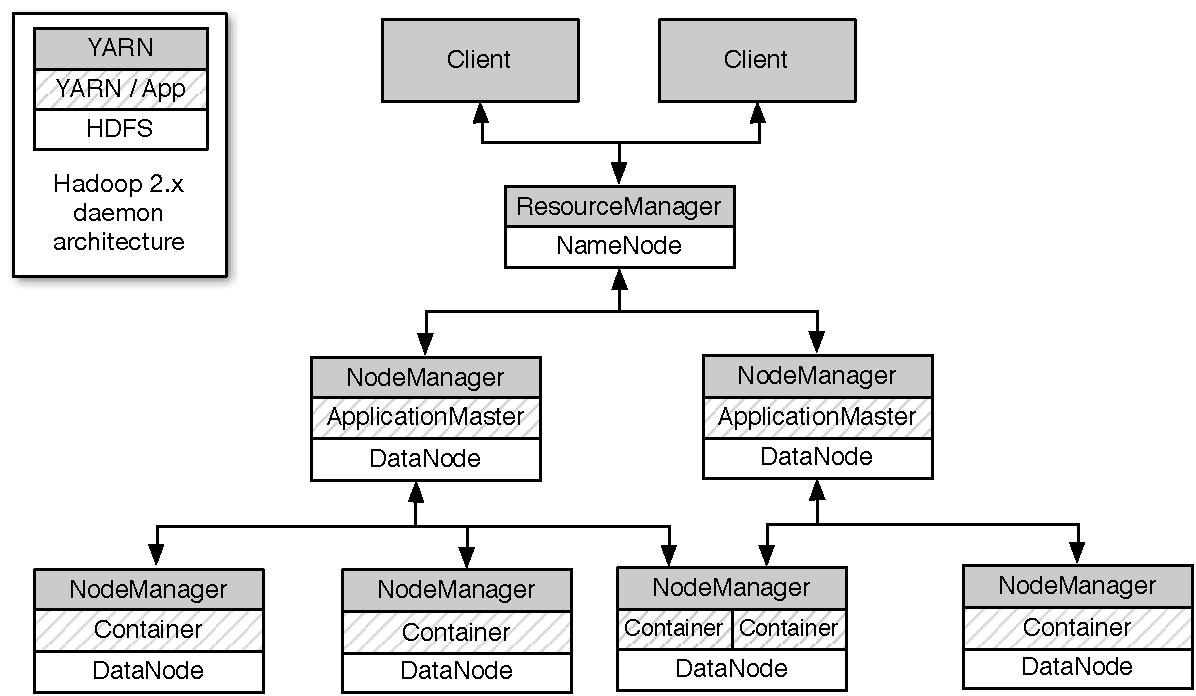
\includegraphics[width=0.85\linewidth]{img/HadoopArch.pdf}
	\caption{Architecture de base de Apache Hadoop 2.x}
	\label{fig:ArquiteturaHadoop}
\end{figure}


On observe donc que le framework Hadoop utilise deux niveaux d'ordonnancement. Les "jobs" représentent des instances avec une granularité plus grande, alors que les tâches représentent des instances de plus fin grain présentes au sein d'un job. 

L'ordonnancement au niveau des jobs est effectué par le \textit{ResourceManager}, la seule entité qui a une vue globale des ressources du système grâce aux informations envoyées par les \textit{NodeManager}. Grâce à ces informations, le \textit{ResourceManager} peut arbitrer la répartition des ressources entre les applications, en se basant sur différentes métriques telles que l'utilisation des ressources, l'équité, les contrats SLA, etc. Un \textit{ApplicationMaster} est ainsi détaché pour chaque application et devient responsable par l'ordonnancement et l'exécution des tâches de cette application par le biais des \textit{conteneurs}, des unités de calcul isolées et disposant d'un accès limité aux ressources (mémoire, CPU). 

Vu cette complexité, le \textit{ResourceManager} a été projeté de manière à pouvoir être optimisé selon contraintes et paramètres des utilisateurs, grâce à un mécanisme d'extensions. Toutefois, la plupart des utilisations répertoriées dans la littérature n'utilisent que les ordonnanceurs livrés avec Hadoop. Le plus simple de ces algorithmes d'ordonnancement est le \textit{Internal Scheduler}, une simple liste d'exécution où les jobs sont servis selon leur ordre d'arrivée (FIFO). Évidemment, cet algorithme n'est indiqué que pour les \textit{clusters} où la compétition pour des ressources n'est pas un problème. 

Deux autres algorithmes sont souvent cités : l'algorithme \textit{Fair Scheduler} et l'algorithme \textit{Capacity Scheduler}. \textit{Fair Scheduler} utilise un mécanisme d'ordonnancement à deux niveaux pour effectuer un partage équitable entre des jobs de petite taille \cite{Hadoop}. \textit{Capacity Scheduler}, de son côté, a été créé pour l'utilisation de Hadoop dans un environnement où plusieurs partenaires contribuent afin de composer un grand \textit{cluster}. En effet, le \textit{Capacity Scheduler} offre des garanties minimales d'accès aux ressources pour chaque partenaire, tout en permettant l'utilisation élargie du \textit{cluster} lorsque des ressources se trouvent libres \cite{Hadoop}.

Les trois algorithmes cités ci-dessous illustrent des approches différentes pour la gestion des jobs, mais cela se fait uniquement par rapport à des facteurs tels que la disponibilité de ressources ou les politiques d'équité, sans jamais prendre en compte la dynamicité et l'hétérogénéité de l'environnement d'exécution. En effet, Hadoop considère que la gestion à grain fin de l'exécution incombe au  \textit{ApplicationMaster}, qui a une vue plus proche de l'application mais qui est aussi limité aux ressources que lui sont attribués au départ.

Malheureusement, le fonctionnement de l'\textit{ApplicationMaster} est peu documenté. Afin de combler ce manque d'information, nous avons analysé son code source et conduit des expériences pour comprendre ses politiques d'allocation des tâches (résultats publiés dans \cite{UBICOMM2014}). Ce que ressort est un simple mécanisme de remplissage des n{\oe}uds visant la proximité des tâches : on remplit un n{\oe}ud avec autant de conteneurs qu'il peut supporter, pour ensuite commencer re remplissage du prochain n{\oe}ud.   

Ceci nous a permis aussi d'observer que l'\textit{ApplicationMaster} se limite à répartir les conteneurs sans une véritable adéquation au contexte d'exécution. Toute connaissance sur la capacité des n{\oe}uds provient du \textit{ResourceManager}, la seule entité qui est alimentée avec ces informations. Ainsi, la modification des algorithmes d'ordonnancement dans le but d'inclure des informations de contexte doit se faire en étroite relation avec le \textit{ResourceManager}.



\section{Dynamicité des Ressources dans Hadoop} \label{sec:related}

La littérature propose différentes approches pour rendre Hadoop plus compatible avec les environnements hétérogènes. Des travaux comme \cite{Kumar2012}, \cite{Tian2009} ou \cite{Rasooli2012} assument que les applications \textit{MapReduce} sont exécutées régulièrement dans un environnement de "production", et que chacune des applications a des besoins spécifiques en CPU, mémoire, réseaux ou en stockage. Cette hypothèse considère donc la possibilité d'optimiser l'exécution des application en faisant la correspondance entre les besoins et les caractéristiques des ressources. De même, \cite{Isard2009} propose un algorithme d'ordonnancement où une fonction de coût basée sur un graphe "capacité-demande" permet l'ordonnancement des jobs.

Les travaux cités ci-dessus considèrent des ressources hétérogènes mais statiques et, une fois lancés, ces jobs ne sont plus "suivis" car l'environnement est supposé immuable. Une manière de rendre cet ordonnancement plus dynamique est d'incorporer des informations sur le déroulement des tâches. Par exemple, \cite{Zaharia2008} et \cite{Chen} essayent d'améliorer la distribution des tâches afin de réduire le temps de réponse dans des \textit{clusters} de grande taille. Pour cela, \cite{Zaharia2008} utilise des heuristiques pour estimer la progression des tâches et ainsi décider s'il faut lancer des tâches spéculatives. Les tâches spéculatives sont des doublons (ré-soumissions) qui sont lancées lorsqu'il y a la soupçon qu'une tâche originale est retardée à cause d'un n{\oe}ud défaillant ou trop lent. Dans une ligne similaire, \cite{Chen} propose l'utilisation des traces historiques d'exécution afin d'aider cette décision. 


Une autre manière d'augmenter la performance passe par un meilleur placement des données et par l'utilisation de cette information pour le déploiement des jobs \cite{Xie2010}. En faisant un placement optimisé des données, on réduit les transferts de données occasionnés par le lancement de tâches spéculatives sur d'autres n{\oe}uds. Une approche similaire est présentée par \cite{Cavallo2015}, qui étudie les problèmes d'ordonnancement et répartition des données dans les \textit{clusters} géographiquement distribués. Ainsi, ces auteurs présentent un mécanisme d'ordonnancement basé sur les ressources de calcul mais aussi sur le débit du réseau.  

Sans aucun paramètre supplémentaire, les mécanismes cités jusqu'à présent ont comme résultat un équilibrage de charge, obligeant les n{\oe}uds les plus rapides à travailler plus et les moins performants à exécuter moins de tâches. Une manière de rompre cette logique est utilisée par \cite{Sandholm2010},  qui permet d'influencer l'ordonnancement grâce à des profils d'exécution suggérés par l'utilisateur (par exemple, privilégier les n{\oe}uds lents si le job n'est pas prioritaire).  

Il faut observer cependant que la difficulté à adapter l'exécution de \textit{MapReduce} sur des environnements hétérogènes (et dynamiques) est en grand partie due à la conception même de la plate-forme Apache Hadoop, qui est très hiérarchique (voir Figure \ref{fig:ArquiteturaHadoop}). Certains travaux essayent de s'affranchir de ces barrières en développant d'autres plates-formes compatibles avec \textit{MapReduce} mais plus adaptées à l'a dynamicité des ressources.  L'utilisation de overlays P2P est ainsi un choix naturel, comme le montrent \cite{Marozzo2012} et \cite{Steffenel20151034}. Dans le système proposé par \cite{Marozzo2012}, les n{\oe}uds incarnent les différentes fonctions de l'architecture Apache Hadoop (NameNode, etc.) selon les besoins de l'application. Cependant, ce travail vise la tolérance aux fautes et n'explore pas les possibilités d'optimisation de l'ordonnancement des jobs et des tâches. 

L'approche adoptée par la plate-forme CloudFIT \cite{Steffenel20151034} est différente car même si elle repose aussi sur un overlay P2P, on n'essaye pas d'imiter le fonctionnement de Hadoop. CloudFIT est une plate-forme générique de calcul distribué, où des tâches Map et Reduce sont distribuées aux n{\oe}uds de façon opportuniste, selon un mécanisme "bag of tasks". Cette distribution est aussi guidée un ordonnancement guidé par le contexte des ressources et par des profils d'exécution fournis par les applications. Nous détaillerons le fonctionnement de CloudFIT dans le chapitre suivant.

Il faut aussi noter que, à l'exception de CloudFIT, les travaux cités précédemment ne tiennent pas compte de l'évolution des ressources au fil de l'exécution : les ressources sont décrites mais pas observées. Malgré la diversité de travaux sur l'importance de la prise en compte du contexte d'exécution \cite{Baldauf, Maamar, Ramakrishnan2014, Najar2015}, Hadoop reste essentiellement une plate-forme statique. Pour toutes ces raisons, une partie de notre travail au sein du projet STIC-AmSud PER-MARE a été d'intégrer les informations de contexte à l'exécution de Hadoop.

\section{Ordonnancement Orienté par le Contexte} \label{sec:desenv}

Comme indiqué dans la section \ref{subsec:ordoHadoop}, l'élément central de l'ordonnancement est le \textit{Resource Manager}. En effet, c'est grâce aux informations fournies par cet élément que les ordonnanceurs de Hadoop tels que le \textit{Capacity Scheduler} décident du démarrage et du placement des tâches. 

L'implémentation par défaut de Hadoop considère qu'un \textit{NodeManager} déclare ses ressources au \textit{ResourceManager} lors de sa connexion au réseau Hadoop, or la description de ces ressources est usuellement obtenue à partir de fichiers de configuration statiques. Afin de rendre cette information de contexte dynamique, nous devons mettre en place un mécanisme de capture de contexte et aussi permettre au \textit{NodeManager} de communiquer périodiquement ses ressources au \textit{ResourceManager}. 

Afin de modifier le moins possible le code de Hadoop, nous avons développé un module de capture de contexte qui peut être greffé à Hadoop et ainsi mettre à jour les informations sur les ressources disponibles. Les sous-sections suivantes détaillent le fonctionnement de ce module et aussi le mécanisme retenu pour son intégration à Hadoop.

\subsection{Le Collecteur de Contexte\label{sec:gestionnairecontexte}}
Par défaut, Hadoop obtient des informations sur les ressources des n{\oe}uds à partir de fichiers de configuration au format XML. Ces fichiers contiennent plusieurs paramètres, dont le nombre d'unités d'exécution (c{\oe}urs de calcul) et la capacité de la mémoire des n{\oe}uds. Une fois lues, ces informations ne sont pas mises à jour, sauf en cas de redémarrage du n{\oe}ud. Afin de rendre possible l'exécution de Hadoop dans un environnement pervasif, nous avons mis en place un mécanisme de collecte d'informations de contexte qui peut être utilisé pour ajourner la base de connaissances du \textit{ResourceManager}.

Ce collecteur de contexte a été développé dans le cadre du projet PER-MARE\cite{PER-MARE} et est structuré selon le diagramme de classes présenté en Figure \ref{fig:CollectorDiag} \cite{UBICOMM2014}. La capture des différents éléments de contexte se font grâce à l'API standard Java Monitoring API \cite{Oracle}, qui permet l'accès aux caractéristiques de la machine virtuelle Java et de la machine hôte. En effet, cela nous permet d'obtenir des informations de contexte telles que le nombre de processus (c{\oe}urs de calcul), la mémoire du système, ou la charge de ma machine. Le collecteur de contexte a été structuré avec un ensemble d'interfaces et de classes abstraites, ce qui permet de généraliser le processus de la collecte des données. De plus, en raison de sa conception, il est simple d'intégrer des nouveaux collecteurs et ainsi diversifier les informations de contexte.

\begin{figure}[!ht]
	\centering
	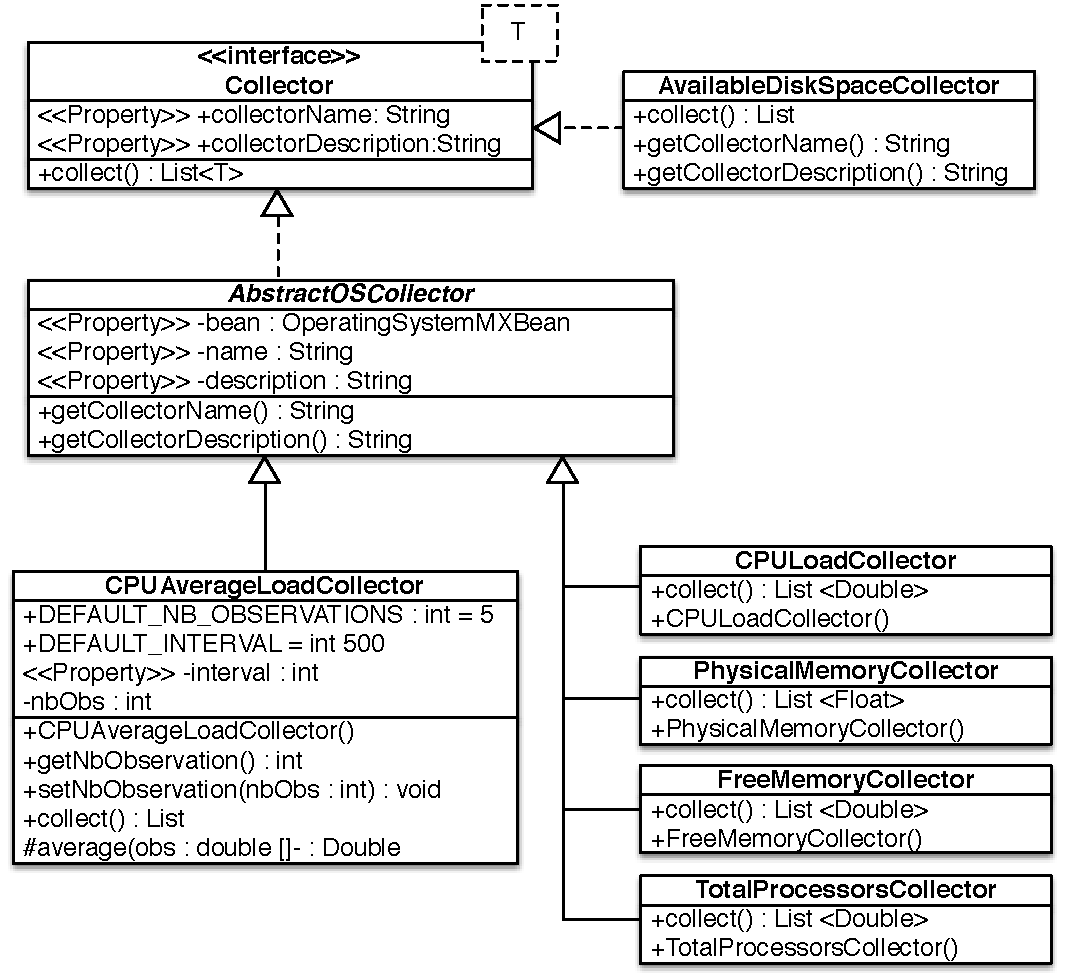
\includegraphics[width=0.75\linewidth]{img/CollectorUML2.pdf}
	\caption{Structure du collecteur de contexte}
	\label{fig:CollectorDiag}
\end{figure}

Cependant, il ne suffit pas de remplacer les fichiers de configuration XML par les informations du collecteur car ces informations resteraient statiques. Afin d'ajourner le \textit{ResourceManager}, il faut que le collecteur de contexte de chaque n{\oe}ud puisse communiquer son état au \textit{ResourceManager}, et cela à n'importe quel moment de l'exécution. Afin de rendre ceci possible, nous avons étendu les possibilités de communication entre le \textit{ResourceManager} et les \textit{NodeManager}, comme expliqué dans la section suivante.    

\subsection{Communication}
Dans l'architecture Hadoop, les informations de contexte collectées par les n{\oe}uds esclaves (\textit{NodeManager}) doivent être transmises au n{\oe}ud maître (\textit{ResourceManager}), qui sera en charge de l'ordonnancement. Au lieu de créer un mécanisme séparé, nous avons choisi d'intégrer cette communication au sein de l'API ZooKeeper \cite{Hunt2010}, qui fait partie de l'écosystème Hadoop. Dans notre cas, les services de ZooKeeper seront utilisés pour récupérer les informations de contexte et les rendre disponible auprès le \textit{ResourceManager}. 

\begin{figure}
	\centering
	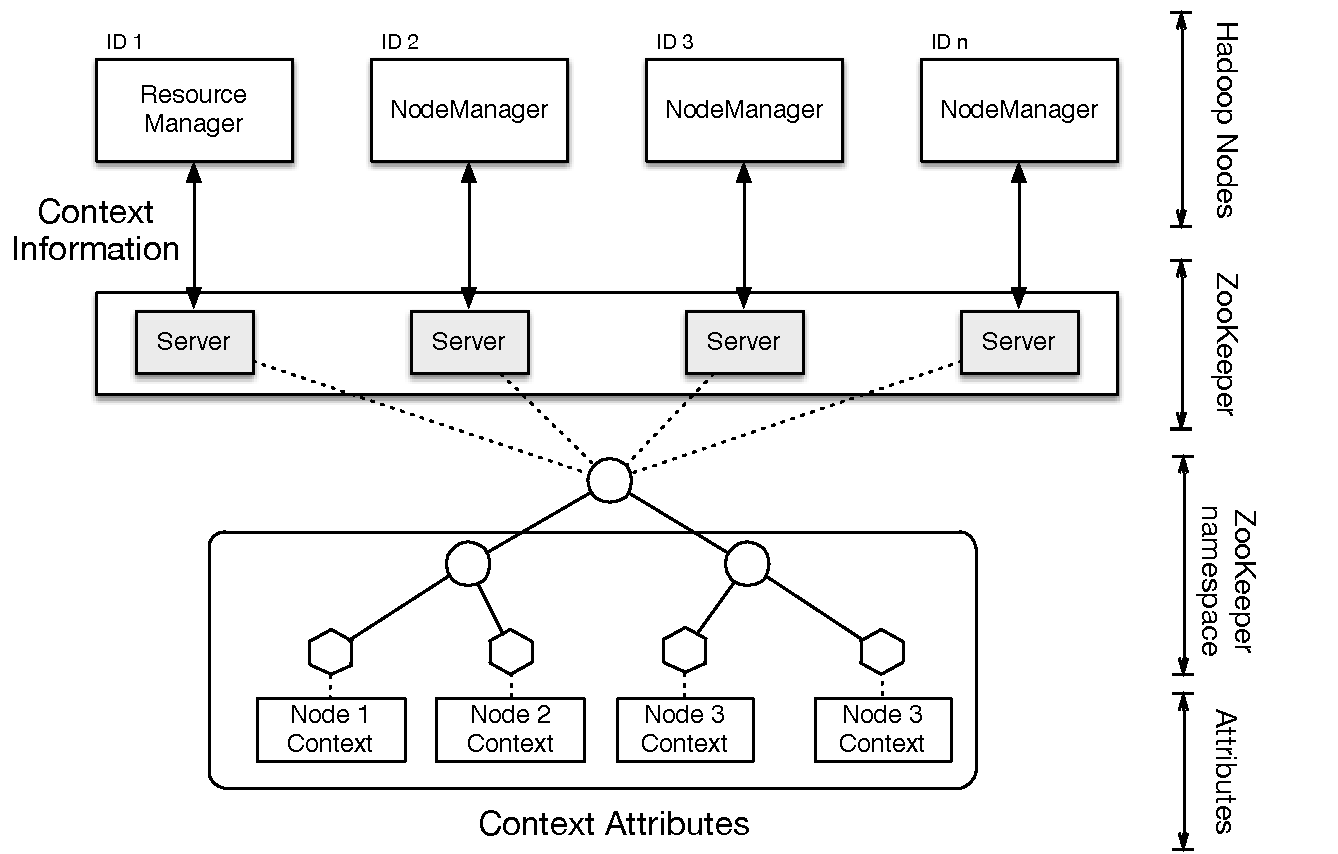
\includegraphics[width=1\linewidth]{img/Zookeeper} 
	\caption{Utilisation de ZooKeeper pour distribuer l'information de contexte\label{fig:zookeeper}}
\end{figure}


Comme illustré en Figure \ref{fig:zookeeper}, tous les esclaves (\textit{NodeManager}) exécutent une instance du service \textit{NodeStatusUpdater}, lequel collecte régulièrement les données sur la disponibilité des ressources (par exemple, à chaque 30 secondes). Si les ressources varient plus qu'un certain seuil/plafond, le tableau dans ZooKeeper sera mis à jour. Ce seuil/plafond est nécessaire car le système d'exploitation peut subir des légères variations des ressources (par exemple, la quantité de mémoire disponible) alors que ces variations n'ont pas un impact sur la capacité d'un n{\oe}ud. Ce mécanisme contribue aussi pour réduire la quantité d'informations échangées et évite trop d'événements qui pourrait impacter la performance de l'algorithme d'ordonnancement. 

De manière similaire, le maître (\textit{ResourceManager}) crée aussi un service pour surveiller les informations sur de ZooKeeper. Lorsque ZooKeeper détecte une modification des données, le maître sera notifié et pourra mettre à jour les informations utilisées par l'ordonnanceur. Les modifications apportées au code source du \textit{ResourceManager} et des \textit{NodeManager} est assez limitée, permettant son application sur différentes versions de Hadoop.

Dans la section suivante nous allons montrer les résultats de quelques expériences faites pour valider ce mécanisme.


\section{Évaluation Pratique} \label{sec:exper}

Afin d'évaluer l'impact de la prise en compte du contexte dans le cadre de l'ordonnancement des tâches, nous avons conduit une série d'expériences sur un petit \textit{cluster} dédié. Cet environnement nous permet de contrôler les ressources disponibles et aussi ceux "observés" par le framework Hadoop, de manière à pouvoir mesurer l'impact d'une mauvaise détection et les avantages de l'adaptation au contexte. Dans les tests effectués, nous avons observé le comportement de Hadoop selon deux métriques, la ressource "mémoire disponible" et le nombre de c{\oe}urs de calcul (\textit{v-cores}). Ces paramètres sont toujours renseignés au \textit{ResourceManager} et font partie des principaux attributs utilisés par l'algorithme Capacity Scheduler. En effet, la mémoire totale disponible et le nombre de c{\oe}urs permettent la définition du nombre de tâches simultanées (conteneurs) qui peuvent être exécutées par un n{\oe}ud. Une mauvaise information peut donc créer une surcharge de la machine, affectant la performance.  

Pour la définition des scénarios d'exécution, nous avons travaillé avec l'hypothèse que la performance est dégradée si la mémoire disponible annoncée au gestionnaire de ressources est supérieure à celle réellement disponible. La situation contraire (plus de mémoire disponible que celle annoncée) n'impacte pas l'exécution d'une tâche. Ainsi, nous avons défini 4 situations d'exécution :

\begin{description}
	\item[Scénario A :] dans ce scénario "de contrôle" la mémoire disponible annoncée au gestionnaire de ressources correspond à la mémoire disponible. De même, le nombre de c{\oe}urs de calcul renseigné correspond au nombre de c{\oe}urs disponibles. Les ressources ne varient pas pendant l'exécution, ce qui peut être considéré comme le "best case". 
	\item[Scénario B :] dans ce cas, la mémoire disponible et le nombre de c{\oe}urs sont inférieurs à ceux annoncés. Cependant, elle ne sera pas mise à jour au niveau du gestionnaire de ressources, reproduisant ainsi le comportement par défaut de Hadoop. Comme l'ordonnanceur ne s'adapte pas, ceci peut être considéré comme un scénario "worst case".
	\item[Scénario C :] dans ce troisième cas, le collecteur de contexte est actif dès le départ et renseigne les ressources effectivement disponibles à chaque 30 secondes. Ainsi, quand l'application est lancée, l'ordonnanceur est au courant du contexte d'exécution et peut lancer les tâches conformément à ces ressources, sans surcharger les machines. 
	\item[Scénario D :] finalement, ce scénario représente une extension du Scénario C dans lequel l'exécution de l'application \textit{MapReduce} démarre avant la mise à jour du collecteur de contexte. De cette manière l'ordonnanceur est initialisé avec des informations incorrectes et doit s'adapter pendant l'exécution. Cette adaptation n'est pas immédiate car elle ne concerne que l'ordonnancement des tâches en attente, pas celle des tâches déjà en exécution.
\end{description}


\subsection{Benchmarks et Environnement de Tests}

Deux types différents d'application ont été utilisés comme benchmarks afin de vérifier l'impact de l'adaptation au contexte. Même si les applications \textit{big data} sont fortement dépendantes de l'accès mémoire, d'autres facteurs comme l'utilisation de la CPU ou les opérations d'entrée/sortie (I/O) sont aussi importantes. Pour cela, les deux applications choisies ont des profils différents par rapport à leurs besoins en mémoire, CPU et  I/O \cite{Benchmarks}, comme indiqué ci-dessous :
\begin{itemize}
	\item TeraSort: L'application TeraSort \cite{TeraSort2008} est une application destinée à effectuer le tri d'un grand ensemble de données. C'est un benchmark très populaire car les algorithmes de tri stressent la mémoire et la CPU au même temps qu'ils sollicitent l'I/O à cause des masses des données à trier ;
	\item TestDFSIO: Le benchmark TestDFSIO a été conçu spécifiquement pour étudier l'interaction de Hadoop avec HDFS, permettant la découverte de goulots d'étranglement au niveau du réseau d'interconnexion, du système d'exploitation et de la configuration Hadoop. Dans cette application, la mémoire et la CPU sont moins sollicitées.
\end{itemize}

Les deux benchmarks font partie de la plate-forme de tests HiBench \cite{HiBench}. Le tri TeraSort a été exécuté sur un ensemble de données de 15 GB, alors que TestDFSIO a été exécuté avec 90 fichiers de 250 MB chacun. Les différents scénarios ont été exécutés sur la plate-forme Grid'5000 \cite{g5k}. Nous avons configuré un réseau dédié avec 5 machines (dont une "maître" et quatre "esclaves"), chacune avec la configuration suivante : 2 Intel Xeon CPU E5420 @ 2.50 GHz (8 c{\oe}urs par n{\oe}ud) et 8 GB de mémoire RAM. Tous les n{\oe}uds exécutent Ubuntu-x64-12.04, avec JDK 1.7 et la distribution Apache Hadoop 2.5.1. 

L'analyse des performances se fait grâce à l'étude des fichiers de log de chaque tâche (conteneur), qui contiennent des informations sur le n{\oe}ud d'allocation, le moment de démarrage et le temps nécessaire pour l'exécution de chaque tâche. Nous avons choisi d'exécuter les tâches "maître" sur un n{\oe}ud séparé afin de ne pas surcharger les n{\oe}uds esclaves avec des activités de gestion de Hadoop. 

Finalement, afin d'émuler la réduction des ressources en mémoire et c{\oe}urs de calcul nécessaires aux scénarios B, C et D, nous avons choisi de réduire le nombre effectif de n{\oe}uds utilisés, une méthode drastique mais plus fiable que la limitation logicielle des ressources disponibles.

\subsection{Résultats\label{sec:5.4}} 

Les exécutions des benchmarks dans les différents scénarios sont représentées par les diagrammes de Gantt des Figures \ref{fig:gantts} et \ref{fig:DFSIO}, respectivement pour TeraSort et TestDFSIO. De même, les Tableaux \ref{tab:resumo} et \ref{tab:DFSIO} résument les données clés de ces expériences, avec le temps total d'exécution des tâches \textit{map}, le temps moyen d'exécution, l'écart type, le nombre de tâches \textit{map} et aussi le nombre de tâches spéculatives démarrées.  

\begin{figure*}[!ht]
	\centering
	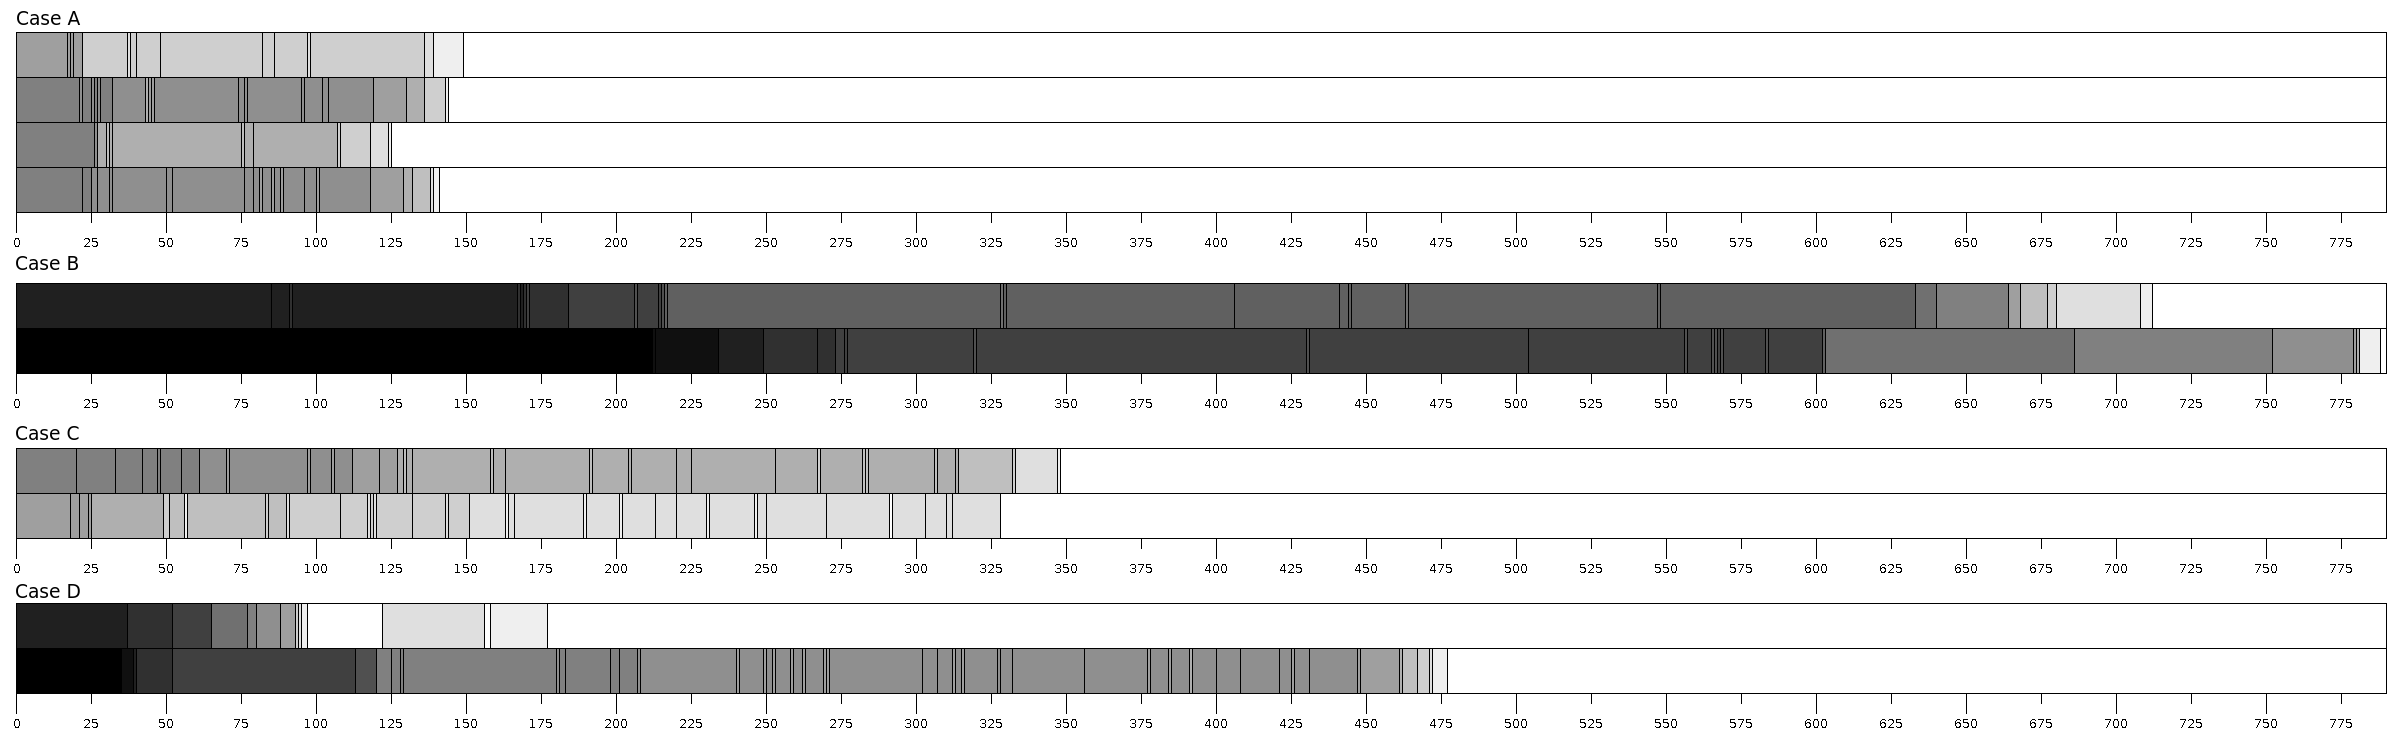
\includegraphics[width=1\textwidth]{img/todos}
	\caption{Diagramme de Gantt pour l'exécution de TeraSort}
	\label{fig:gantts}
\end{figure*}

\begin{figure*}[!ht]
	\centering
	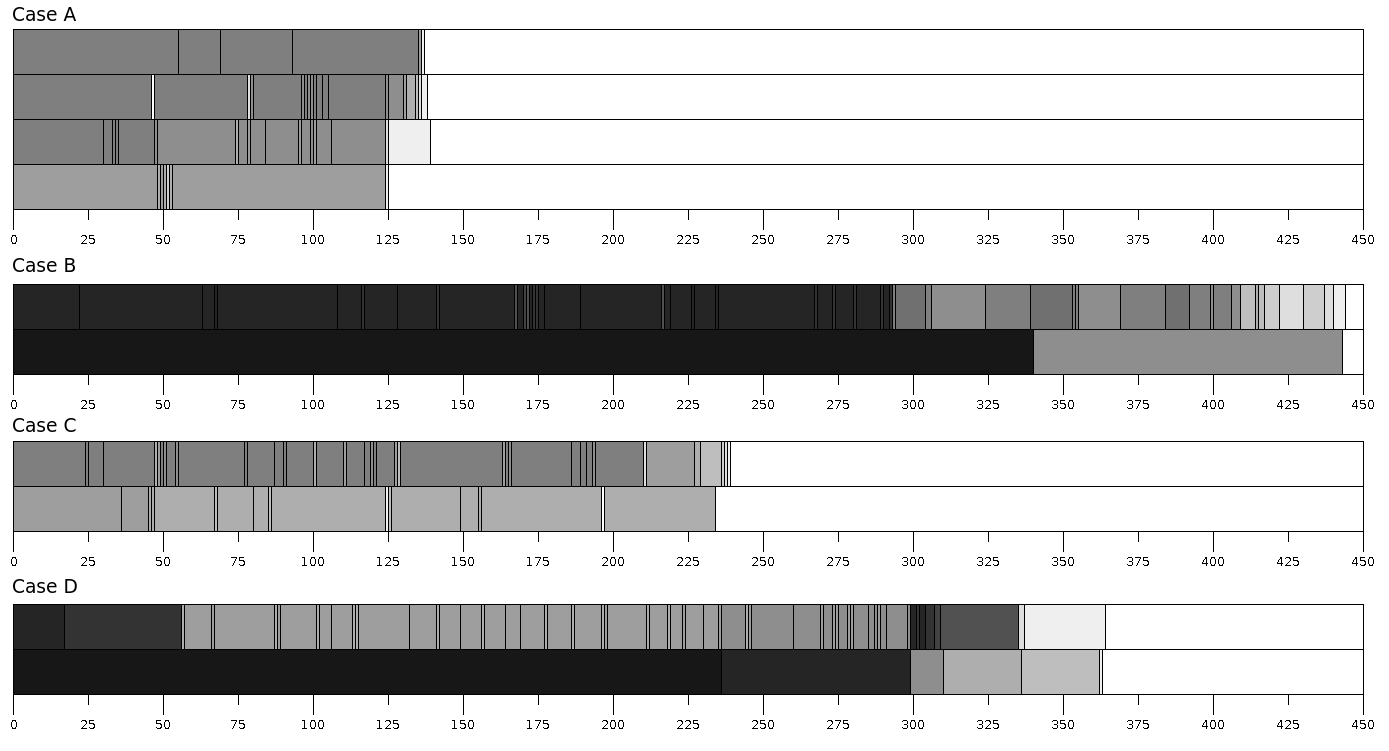
\includegraphics[width=1\textwidth]{img/todos-DFSIO}
	\caption{Diagramme de Gantt pour l'exécution de TestDFSIO}
	\label{fig:DFSIO}
\end{figure*}


\begin{table}
	\caption{Tableau récapitulatif de l'exécution de TeraSort} \label{tab:resumo}
	\centering
	\begin{tabular*}{0.6\hsize}{lllll} 
		\textbf{Scénario} & \textbf{A} & \textbf{B} & \textbf{C} & \textbf{D}\\
		\hline
		Temps total \textit{map} ({\it{s}}) & 149 & 788 & 348 & 477 \\
		Temps moyen ({\it{s}}) & 39.47 & 222.97 & 38.38 & 68.42 \\
		Écart type & 15.73 & 59.86 & 18.09 & 29.91 \\
		\# tâches \textit{map} & 76 & 76 & 76 & 76 \\
		\# tâches spéculatives & 2 & 1 & 3 & 1 \\
	\end{tabular*}
\end{table}

\begin{table}
	\caption{Tableau récapitulatif de l'exécution de TeraSort} \label{tab:DFSIO}
	\centering
	\begin{tabular*}{0.6\hsize}{lllll} 
		\textbf{Scénario} & \textbf{A} & \textbf{B} & \textbf{C} & \textbf{D}\\
		\hline
		Temps total \textit{map} ({\it{s}}) & 139 & 444 & 239 & 364 \\
		Temps moyen ({\it{s}}) & 38.95 & 85.01 & 32.20 & 81.62 \\
		Écart type  & 17.20 & 69.08 & 8.30 & 73.60 \\
		\# tâches \textit{map} & 90 & 90 & 90 & 90 \\
		\# tâches spéculatives & 0 & 9 & 0 & 1 \\
	\end{tabular*}
\end{table}


Pour les diagrammes de Gantt, chaque scénario est composé de 2 ou 4 lignes correspondant au nombre de n{\oe}uds utilisés. Comme indiqué précédemment, les scénarios B, C et D n'utilisent que la moitié des n{\oe}uds du scénario A afin de simuler la réduction des ressources. L'échelle de couleurs présent dans chaque ligne indique la surcharge des n{\oe}uds : plus sombre est le créneau, plus de conteneurs s'exécutent simultanément. De cette manière, un créneau "blanc" n'a aucun conteneur en exécution, alors qu'un créneau "noir" en contient 16 conteneurs (le double de la capacité d'un n{\oe}ud). Les séparations des créneaux indiquent soit le démarrage d'une tâche, soit une fin d'exécution, mais ne permettent pas de suivre le temps d'exécution d'une tâche précise. 

L'analyse des tableaux permet d'identifier certaines tendances. En effet, toutes les exécutions présentent un motif similaire quand on observe le temps total d'exécution : le scénario A est toujours le plus rapide, suivi de des cas C et D puis finalement  B. Nous observons aussi que les scénarios A et C ont les plus petits temps moyens et les plus petites variations de performance, indépendamment de l'application. Ceci s'explique par le fait que dans ces deux scénarios les n{\oe}uds ne sont jamais surchargés car l'ordonnanceur a des informations précises au moment du démarrage de l'application. Ceci s'observe aussi par la tonalité des créneaux, indiquant un nombre moins important de tâches en simultané. Le temps total d'exécution du scénario C est aussi deux fois plus important que celui du scénario A, une conséquence attendue à cause de la réduction des ressources. 

L'analyse du nombre de tâches spéculatives apporte aussi quelques renseignements. Dans le cas de TeraSort, tous les scénarios se comportent de manière similaire. Par contre, dans le cas de TestDFSIO le déploiement de tâches spéculatives ne se fait que lorsque le système est surchargé (notamment dans le scénario B). La raison pour cette différence vient des facteurs qui sont liés au lancement de tâches spéculatives : une tâche spéculative n'est lancée que seulement après le lancement de toute autre tâche "originale", et déclenchée seulement lorsque ces tâches sont en exécution depuis un certain temps (au moins une minute) et n'ont pas progressé autant que la moyenne des autres tâches du job. Dans le cas de TeraSort, les tâches dépendent autant de la mémoire que de la CPU et de l'I/O, et le recouvrement de ces besoins compense d'une certaine manière le manque d'une ressource. TestDFSIO, à l'opposé, s'appuie sur des ressources plus spécifiques et est donc plus enclin à la surcharge des n{\oe}uds. Et même dans les scénarios surchargés, l'utilisation d'un mécanisme de détection du contexte sur le scénario D permet à l'ordonnanceur de lisser la charge lors de la mise à jour des informations sur les ressources.

Il faut aussi pointer un détail concernant les diagrammes de Gantt. Dans tous les benchmarks il y a un n{\oe}ud qui semble moins chargé que les autres. Ceci n'est pas la faute à une mauvaise répartition de la charge mais plutôt à la présence de tâches \textit{reduce}, qui ne sont pas affichées dans les diagrammes. En effet, Hadoop permet le démarrage de tâches \textit{reduce} aussitôt un certain nombre de tâches \textit{map} a été complété, ce qui est le cas pour ces applications.



\section{Travaux en Cours et Perspectives} \label{sec:disc}

Dans ce chapitre j'ai essayé de mettre en évidence l'importance de la prise en compte des variations dynamiques des ressources. L'adaptation au contexte est une discipline essentielle à d'autres domaines tels que les applications mobiles, les réseaux sociaux et les systèmes d'information pervasifs, mais cela n'est pas encore ancré comme une pratique courante dans le calcul haute performance ni même dans les outils \textit{big data} les plus populaires. 

Le résultat de ces expériences démontre que l'utilisation d'un mécanisme de collecte et de mise à jour des informations de contexte permet l'adaptation de l'ordonnanceur Hadoop aux aléas d'une plate-forme d'exécution dynamique. La solution que nous avons proposé dans ce travail permet non seulement un gain de performance dans les scénarios avec risque de surcharge mais aussi impose très peu de modification au niveau du code source de Hadoop, rendant la solution suffisamment générique et intégrable aux différentes versions de ce framework. 

Il faut aussi citer un deuxième travail effectué en parallèle à celui présenté ici. Aussi dans le cadre du projet PER-MARE, ce travail s'est porté sur une autre élément critique de la version 1.x de Hadoop, le \textit{JobTracker}. Contrairement au \textit{RessourceManager} de Hadoop 2.x, la version 1 de Hadoop a un élément centralisé qui n'est pas tolérant aux pannes (c'est un \textit{single point of failure}). Si le processus exécutant le \textit{JobTracker} disparâit, aucune nouvelle soumission sera exécutée et à terme les n{\oe}uds esclave n'auront plus aucun travail à exécuter. Le travail que j'ai conduit avec en collaboration avec l'équipe de l'Universidad de la República (Uruguay) consistait à mettre en place une sauvegarde des paramètres du \textit{JobTracker} sur ZooKeeper, et de faire surveiller son état par une machine "backup" choisie par son stabilité. Nous avons pu développer et tester cette fonctionnalité et publier ses résultats \cite{Steffenel2015-WoC, Rey14a}. Malheureusement, l'arrivée de la version 2.x de Hadoop a introduit des modifications qui ont rendu ce travail obsolète. 

Les perspectives de poursuite dans le domaine de la prise en compte du contexte des ressources sont nombreuses et font partie de la plupart de mes objectifs de recherche dans les années à venir. Parmi elles, je pourrais citer :

\subsubsection*{Développement de techniques d'ordonnancement sensibles au contexte}

de même, La suite des travaux vise l'étude des plates-formes de micro-services, on espère bientôt pouvoir effectuer des nouvelles campagnes d'expérimentation.



\subsubsection*{Adaptation d'outils \textit{big data}}

À moyen terme je souhaite apporter des élements de gestion de contexte à la plate-forme Apache Storm. Bien qu'elle n'inclut pas la prise en charge du contexte des ressources, elle dispose d'autres fonctionnalités qui peuvent être utiles dans le cas d'un déploiement \textit{fog computing}, par exemple en tant que plate-forme arrière pour le traitement des flux des dispositifs IoT. De plus, c'est une plate-forme qui repose sur un overlay P2P : son étude peut apporter des idées et optimisations pour la plate-forme CloudFIT que je développe.



